\section{A worked protocol for one elementary step}
\label{sec:worked}

Section~\ref{sec:intro} listed the inputs a certificate needs. This section
supplies them for one system far enough to expose where the method is already
informative and where it is not. Nothing below is a molecular energy
calculation; the certified content is arithmetic on published growth data plus
two geometric inequalities, and the negative result is proved.

\subsection{System and evidence status}

The target is $\mathrm{CaF_2}$ growth from a calcium amidinate and hydrogen
fluoride on the fluorine-terminated $\mathrm{CaF_2}(111)$ cleavage plane.
Every choice below is either taken from a cited measurement or is explicitly
labelled as a modelling decision.

\begin{itemize}
\item \emph{Surface.} The $(111)$ plane is the natural cleavage plane and is
F-terminated with a $(1\times1)$ unreconstructed termination
\citep{Vogt2005,Puchin2001}. Its repeat unit along $[111]$ is a
F--Ca--F trilayer of height $a_0/\sqrt3$ \citep{Calleja2005}. Diffusion of
adsorbed hydrogen and water on alkali-earth fluoride surfaces has been treated
by DFT \citep{Foster2009}, and the morphology of group-II fluoride crystallites
at finite HF partial pressure has been modelled \citep{Kaawar2017}.
\item \emph{Lattice constant.} $a_0 = 5.4626$~\AA, room-temperature XRD powder
data (Swanson \& Tatge, NBS Circular 539 (1953) 69--70; ICSD 52754).
\item \emph{Precursor pair.} Bis($N,N'$-di-\emph{i}-propylformamidinato)calcium(II)
with anhydrous HF, reported at 175--250~$^\circ$C with a growth per cycle of
$0.3$--$0.4$~\AA/cycle \citep{Hennessy2023}.
\item \emph{Precursor nuclearity.} The compound is a \emph{dimer} in the solid
state and is retained in solution, with Ca$\cdots$Ca $=3.323$~\AA, $\mathrm{Ca_2C_{28}H_{60}N_8}$,
$M=589.00$~g\,mol$^{-1}$, monoclinic $P2_1/c$, $V=3754(3)$~\AA$^3$, $Z=4$ at
100~K \citep{Kim2016}. This matters below, because the steric footprint of a
dimer is not that of a monomer.
\item \emph{Adsorbate state.} Periodic DFT places HF \emph{molecularly} on
$\mathrm{CaF_2}(111)$ without dissociation, with $E_{\mathrm{ads}}=-0.40$,
$-0.48$ and $-0.62$~eV at 100\%, 50\% and 25\% coverage, the H hydrogen-bonded
to a surface F \citep{Kaawar2019}. Dissociation to a surface bifluoride
$\mathrm{FHF^-}$ is reported on $(100)$, not $(111)$.
\item \emph{Competing routes in the literature.} $\mathrm{Ca(thd)_2}$ with
$\mathrm{TiF_4}$ at 300--450~$^\circ$C \citep{Pilvi2007,Pilvi2008}; HF--pyridine
as a fluorine co-reactant \citep{Lee2016}; the first metal-fluoride ALD
process \citep{Ylilammi1994}; and, importantly, a second class of calcium
process in which the fluorine is carried by the ligand rather than delivered
externally: $\mathrm{Ca(hfac)_2}$ (calcium hexafluoroacetylacetonate, six
fluorines on the $\beta$-diketonate) with $\mathrm{O_3}$ at 300~$^\circ$C,
giving $0.3$~\AA/cycle and a Rutherford-backscattering stoichiometry of
$\mathrm{CaF_{2.17}}$ with under 5~at\% oxygen \citep{Putkonen2011}. The same
work reports the reverse order, oxide growth from a non-fluorinated
$\beta$-diketonate followed by fluorination with Hhfac and $\mathrm{O_3}$,
which it judges more feasible and which leaves oxygen below the 2~at\%
detection limit. The volatility of such fluorinated diketonates, and the
solid--gas equilibrium governing precursor transport, are non-trivial in their
own right \citep{LoPresti2022}. Reviews of the field are
\citep{Atosuo2024,Hennessy2017}.
\end{itemize}

The general mechanism is better constrained than it first appears, even though
nothing is known specifically for this precursor pair. In situ quartz-crystal
microbalance and infrared work on $\mathrm{AlF_3}$ from $\mathrm{Al(CH_3)_3}$ and
HF finds that the HF pulse both protonates the metal--ligand bond
($\mathrm{HF}+\mathrm{M{-}CH_3}\to\mathrm{M{-}F}+\mathrm{CH_4}$) \emph{and}
leaves molecular HF adsorbed as a surface fluorine reservoir whose coverage
fixes the cycle stoichiometry \citep{Lee2015}. The same scheme is written for
$\mathrm{ZrF_4}$ from a tetrakis(ethylmethylamido)zirconium precursor, where the
volatile byproduct is the free amine \citep{Lee2016}. Protonating an amidinate
likewise gives the conjugate amidine, and amidine desorption has been observed
from a metal surface, together with re-adsorption that is a known carbon
contamination route \citep{Ma2011}.

For the present system, therefore, the expected net reaction is
\[
\mathrm{Ca(amd)_2} + 2\,\mathrm{HF}
  \longrightarrow \mathrm{CaF_2} + 2\,\mathrm{Hamd},
\]
with $\mathrm{Hamd} = N,N'$-di-\emph{i}-propylformamidine. No in situ
mass-balance, infrared, or mass-spectrometric study of this pair exists, and
\emph{no measured or computed activation energy for HF reacting with any metal
amidinate surface has been found}. The only activation energies available for
HF fluorination concern amorphous alumina
($0.18$--$1.14$~eV) \citep{Khumaini2025}; they are not transferable to
$\mathrm{CaF_2}$ and are not used below.

\subsection{Certified arithmetic from published growth data}

Two published numbers, one measured and one geometric, determine the fraction
of a layer deposited per cycle. Let $p$ be the trilayer height and $s$ the
growth per cycle. Writing $s = p\,\theta$ with $\theta$ the fractional coverage, an
interval $s\in[s_1,s_2]$ with $p>0$ gives $\theta\in[s_1/p,\ s_2/p]$
(Lemma~\ref{lem:coverage-lean}).

\begin{lemma}[Interval coverage]
\label{lem:coverage-lean}
For real $p>0$ and $s=p\,\theta$, if $s_1\le s\le s_2$ then
$s_1/p\le \theta\le s_2/p$.
\end{lemma}
\begin{proof}
From $s=p\,\theta$ we get $\theta=s/p$. Since $p>0$, division by $p$ is monotone, so
$s_1/p\le s/p\le s_2/p$.
\end{proof}

With $p=a_0/\sqrt3=3.1538$~\AA{} and $s\in[0.3,0.4]$~\AA/cycle,
\[
c \in \left[\frac{0.3}{3.1538},\ \frac{0.4}{3.1538}\right]
  = [9.51\%,\ 12.68\%].
\]
Each cycle therefore completes about one tenth of a trilayer.

On the unreconstructed F-terminated $(111)$ plane the Ca ions form a triangular
lattice of spacing $a_0/\sqrt2$, so one Ca site occupies
\[
A_{\mathrm{site}} = \tfrac{\sqrt3}{2}\left(\tfrac{a_0}{\sqrt2}\right)^2
= \tfrac{\sqrt3}{4}a_0^2 = 12.9211\ \text{\AA}^2 .
\]
The areal density of deposited Ca follows as
$\sigma = \theta/A_{\mathrm{site}} \in [0.00736,\ 0.00982]$~\AA$^{-2}$, i.e.\ one
deposited Ca per $101.9$--$135.8$~\AA$^2$ of surface. That is $7.9$ to $10.5$
times the area of a bare Ca site.

\begin{remark}
This ratio is the quantitative statement that the cycle is \emph{not} limited
by the availability of surface sites. It does not identify the limiting
mechanism.
\end{remark}

\begin{figure}[t]
\centering
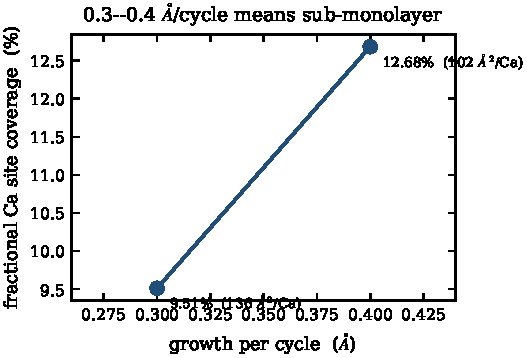
\includegraphics[width=\columnwidth]{fig_coverage}
\caption{Growth per cycle mapped to fractional coverage of Ca sites on the
CaF$_2$(111) surface, using $a_0=5.4626$~\AA{} and a site area of
$12.92$~\AA$^2$. The reported $0.3$--$0.4$~\AA{}/cycle corresponds to
$9.5$--$12.7\%$ of a monolayer, so growth is far from saturating the available
sites. This is arithmetic on published numbers, not a surface calculation.}
\label{fig:coverage}
\end{figure}

\subsection{A geometric design rule for the ligand}

The ratio above invites a purely geometric bound, which holds regardless of
kinetics.

\begin{theorem}[Footprint bound]
\label{thm:footprint}
Let $\sigma>0$ be the number of precursor molecules deposited per unit area and
let $A>0$ be the area each occupies, with no overlap. Then $\sigma A\le1$, and
if $A_0\le A$ for some ligand footprint $A_0>0$ then
\[
\sigma \le \frac{1}{A_0}.
\]
Equivalently, with growth per cycle $s = p\,\sigma A_{\mathrm{site}}$,
\[
s \le \frac{p\,A_{\mathrm{site}}}{A_0}.
\]
\end{theorem}
\begin{proof}
Non-overlap gives $\sigma A\le1$. Dividing by $\sigma>0$ yields
$A\le1/\sigma$; since $A_0\le A$ and both are positive,
$1/A\le1/A_0$, hence $\sigma\le1/A\le1/A_0$. Multiplying
$s=p\,\sigma A_{\mathrm{site}}$ by this bound gives the second inequality.
\end{proof}

The theorem is a cap, not a prediction: it constrains what a cycle can deposit
and says nothing about whether the cycle reaches the cap. Read backwards,
however, it is a design rule. A ligand of footprint $A_0$ caps the growth per
cycle at $pA_{\mathrm{site}}/A_0$, so a bulky ligand cannot produce a high
growth rate no matter how favourable its surface chemistry.

Read backwards a second time, it becomes testable, because $A_0$ can be
measured independently of any growth experiment. The crystal structure of the
dimer \citep{Kim2016} gives a volume per dimer of
$V=3754/4=938.5$~\AA$^3$, implying a crystal density of
$MZ/(N_A V_{\mathrm{cell}})=1.042$~g\,cm$^{-3}$ --- a value ordinary for an
organometallic, which is a useful check that the cell contents were read
correctly. Treating one dimer as a sphere of that volume gives a cross-section
of
\[
A_0 = \pi\left(\frac{3V}{4\pi}\right)^{2/3} = 115.9\ \text{\AA}^2
  \quad (\text{the cube-root estimate } V^{2/3} \text{ gives } 95.9\ \text{\AA}^2),
\]
against the $A_0\le101.9$--$135.8$~\AA$^2$ that the measured growth per cycle
demands. The two independent published datasets agree, both placing the dimer
footprint at about nine times the bare Ca site area of $12.92$~\AA$^2$.

\begin{remark}
This is consistency, not proof, and the distinction is worth stating precisely.
Agreement of two numbers is evidence that the intact dimer is the adsorbing
species and blocks roughly eight to ten Ca sites per cycle. It does not exclude
a kinetic limitation, which would produce the same measured growth; the crystal
structure is measured at 100~K while deposition runs at 175--250~$^\circ$C, so
the footprint could differ; and the model reaction below is computed for a
truncated ligand. What the comparison does do is convert a vague appeal to
``steric hindrance'' into a falsifiable numerical statement: if a future
measurement placed the adsorbed footprint below about $100$~\AA$^2$, steric
self-limitation by the intact dimer would be excluded.
\end{remark}

\subsection{Why sampling cannot certify a barrier}

It is tempting to sample energies at a set of candidate configurations and read
a barrier off their maximum. That inference is not available, and the failure
is elementary.

\begin{theorem}[No upper bound from sampling]
\label{thm:nosampling}
There is a configuration set $X$ with a subset $S\subseteq X$, nonempty, and an
energy function $E:X\to\R$ such that $E=0$ on all of $S$ while
$\max_X E = 10$. Consequently no function of the sampled values
$\{E(x):x\in S\}$ alone bounds $\max_X E$ from above.
\end{theorem}
\begin{proof}
Take $X=\{0,1,2\}$, $S=\{0,2\}$, and $E(0)=E(2)=0$, $E(1)=10$. Then
$\max_S E = 0$ and $\max_X E = 10$, and the sampled data are identical for this
$E$ and for the function that is identically zero, which has maximum $0$. Any
claimed upper bound derived from the samples would therefore have to be at
least $10$ and at most $0$.
\end{proof}

The positive direction survives: a sampled lower bound is valid at every
configuration where it is evaluated, so its maximum over the samples is a valid
lower bound on any barrier whose path passes through those configurations
(Lemma~\ref{lem:sample-lower}).

\begin{lemma}[Lower bound from samples]
\label{lem:sample-lower}
Let $L(x)\le E(x)$ for $x\in S$ and let $E_r\le U_r$. Then for every $x\in S$,
$L(x)-U_r \le E(x)-E_r$.
\end{lemma}
\begin{proof}
Immediate from $L(x)\le E(x)$ and $-U_r\le-E_r$.
\end{proof}

The asymmetry is the reason a certificate must treat the two directions
separately. When the interval produced for a barrier is one-sided, it must be
reported as one-sided.

\subsection{Formal verification}

Lemmas~\ref{lem:coverage-lean} and \ref{lem:sample-lower} and
Theorems~\ref{thm:footprint} and \ref{thm:nosampling} are formalized in Lean~4
against \texttt{mathlib} as \texttt{gpc\_coverage\_interval},
\texttt{barrier\_lower\_from\_samples},
\texttt{max\_density\_from\_ligand\_size} with
\texttt{gpc\_upper\_from\_ligand\_footprint}, and
\texttt{sampling\_gives\_no\_upper\_bound} respectively, together with the
supporting interval lemmas \texttt{adsorption\_energy\_interval},
\texttt{two\_corrections\_widen}, \texttt{coverage\_gpc\_interval},
\texttt{packing\_bound}, \texttt{barrier\_upper\_at\_max},
\texttt{certified\_barrier\_interval}, \texttt{stays\_positive} and
\texttt{certified\_negative}. Each is checked with \texttt{\#print axioms} and
depends only on \texttt{propext}, \texttt{Classical.choice} and
\texttt{Quot.sound}; no \texttt{sorry}, \texttt{admit} or project-defined axiom
appears in the development. Kernel acceptance certifies the inequalities above
given their hypotheses. It certifies nothing about the hypotheses themselves,
which remain physical or geometric inputs.

\subsection{The model reaction, and what its number does not mean}

The protonation step can be computed for a truncated model. Replacing both
di-\emph{i}-propyl groups by hydrogen gives
\[
\mathrm{Ca(formamidinate)_2} + 2\,\mathrm{HF}
 \longrightarrow \mathrm{CaF_2} + 2\,\mathrm{formamidine},
\]
electron-balanced at $66 + 2\times10 = 38 + 2\times24$. Each species was relaxed
until the analytic Hessian had \emph{no imaginary frequency}, which is a stronger
requirement than a small gradient: a vanishing gradient is satisfied by saddle
points as well as minima, and three of the four species were in fact at saddles
when only the gradient was checked (formamidine $-246.8$, $\mathrm{CaF_2}$ $-103.5$,
$\mathrm{Ca(famd)_2}$ $-74.1$~cm$^{-1}$). Displacing along the imaginary mode and
re-relaxing removed them. The reported energies are at geometries converged on the
rotation- and translation-projected gradient, which reaches
$4.5\times10^{-7}$ to $6.9\times10^{-5}$~Ha\,\AA$^{-1}$ for formamidine, HF and
$\mathrm{Ca(famd)_2}$, and $2.9\times10^{-4}$ for $\mathrm{CaF_2}$, whose bend is too
soft to do better. Frequencies were obtained from the analytic
Hessian with translations and rotations projected out, and the conversion was
checked against known spectra (HF $4213.7$~cm$^{-1}$; H$_2$O at $1540.3$,
$3918.7$, $4036.1$~cm$^{-1}$).

\begin{figure}[t]
\centering
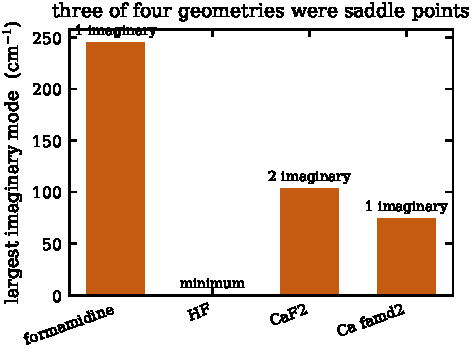
\includegraphics[width=\columnwidth]{fig_imaginary}
\caption{Largest imaginary mode for each of the four species as first optimised,
i.e.\ with the gradient converged but the Hessian unchecked. Three of the four
were saddle points. A small projected gradient is therefore not evidence of a
minimum, and every reported energy in this section was re-verified after the
displacement shown here.}
\label{fig:imaginary}
\end{figure}

Eight functional/basis combinations were evaluated at those minima, and
$\mathrm{CaF_2}$ was treated twice: at its unconstrained minimum and constrained to
$D_{\infty h}$ with only the bond length relaxed. The pair brackets a systematic
error that the spread alone does not see.

\begin{center}
\begin{tabular}{lcc}
\hline
Method & $\Delta E$ bent (kcal\,mol$^{-1}$) & $\Delta E$ linear \\
\hline
PBE/def2-svp     & $-11.95$ & $-9.69$ \\
PBE/def2-tzvp    & $-8.17$  & $-7.02$ \\
PBE/def2-svpd    & $-6.05$  & $-5.69$ \\
PBE/def2-tzvpd   & $-7.05$  & $-6.18$ \\
B3LYP/def2-svp   & $-10.45$ & $-8.98$ \\
B3LYP/def2-tzvp  & $-8.59$  & $-8.19$ \\
B3LYP/def2-svpd  & $-7.11$  & $-7.40$ \\
B3LYP/def2-tzvpd & $-8.16$  & $-8.04$ \\
\hline
spread & $5.90$ & $4.00$ \\
\hline
\end{tabular}
\end{center}

The model reaction is exothermic throughout: the full bracket is
$5.7$--$12.0$~kcal\,mol$^{-1}$, with a method spread of $5.9$ on the bent treatment
and $4.0$ on the linear one. Two systematic effects are visible and neither is a
method spread. First, diffuse functions matter by $4$--$6$~kcal\,mol$^{-1}$: the
four $d$-augmented bases give $-6.1$ to $-8.2$, the four non-augmented $-8.2$ to
$-12.0$. That is expected for a species as polar as $\mathrm{CaF_2}$ and it is why
the augmented levels are the ones to trust. Second, the bent-versus-linear column spans
$0.1$--$2.3$~kcal\,mol$^{-1}$ at these levels, but as the CCSD(T) check above
establishes, that span measures DFT's error in the barrier and not a structural
freedom of the molecule: at a correlated level the two structures are within
$0.15$~kcal\,mol$^{-1}$ of each other. The column is reported because the
calculation was performed in both ways, not because the distinction is physically
worth $2$~kcal\,mol$^{-1}$.

We therefore report the reaction energy as a bracket rather than a number:
$-6$ to $-8$~kcal\,mol$^{-1}$ at the levels we consider adequate
(B3LYP/def2-svpd, B3LYP/def2-tzvpd, PBE/def2-tzvpd), widening to $-5.7$ to
$-12.0$ if the non-augmented levels are admitted. Earlier values from this project,
$-13.4$ to $-10.3$ and then $-11.6$ to $-8.1$, were obtained at saddle-point
geometries and with a basis that over-bends $\mathrm{CaF_2}$ by an order of
magnitude in the barrier; both are withdrawn.

A remark on what the spread does \emph{not} measure. The $\mathrm{CaF_2}$ error
discussed in the previous paragraph is common to all eight levels, so it does not
appear in the $5.9$ or the $4.0$. The spread is a lower bound on the uncertainty,
not an estimate of it.

\paragraph{The bending potential, and a premise we had to withdraw.}
$\mathrm{CaF_2}$ was re-optimised from a bent start; the linear structure is a
saddle, with an imaginary bend at PBE/def2-svp ($-103.5$~cm$^{-1}$), PBE/def2-tzvp
($-154.6$), B3LYP/def2-svp ($-91.5$) and B3LYP/def2-tzvp ($-143.3$~cm$^{-1}$). The
imaginary bend is not a basis artefact, and it is not a grid artefact either: the
harmonic eigenvalue converges from grid level $4$ onward ($-103.5$, $-102.4$,
$-102.8$, $-102.5$~cm$^{-1}$ at levels $4$--$7$), matching an unpruned $(150,770)$
reference to $0.01$~cm$^{-1}$. At coarser levels the sign is not trustworthy
(levels $1$ and $2$ give $+185$ and $+414$~cm$^{-1}$).

We had written that gas-phase $\mathrm{CaF_2}$ is conventionally linear and that
the computed bending is therefore likely an artefact. \emph{That premise is wrong
and is withdrawn.} $\mathrm{CaF_2}$ is quasilinear: a bent equilibrium at
$\theta_e = 154.3^\circ$ behind a barrier of only $54$~cm$^{-1}$
($0.15$~kcal\,mol$^{-1}$) at linearity, with a variational $\nu_2$ of
$9$~cm$^{-1}$ \citep{Koput2004}; CCSD(T) gives $157^\circ$ \citep{Vasiliu2010}, and
a recent CCSD(T)/CASPT2 study classifies $\mathrm{CaF_2}$ as quasilinear at most
temperatures and highly fluxional \citep{Romeu2025}. Molecular-beam electric
deflection establishes a permanent dipole, hence bending on the experimental
timescale \citep{Wharton1963}. No gas-phase angle has been determined: the
frequently quoted $\approx145^\circ$ is a matrix-isolation value that moves by more
than $20^\circ$ between Ar and Kr \citep{Calder1969}.

So the sign of our result is right and its magnitude is not. The \emph{well depth}
is the artefact, not the bending. PBE and B3LYP are reported to over-bend these
systems \citep{Donald2006}, and the barrier we compute is basis-sensitive by nearly
an order of magnitude: $2.19$~kcal\,mol$^{-1}$ at PBE/def2-svp, $1.14$ at
def2-tzvp, $0.50$ at def2-svpd, $0.87$ at def2-tzvpd, $1.52$ at B3LYP/def2-svp and
$0.29$ at B3LYP/def2-tzvpd, against the $0.15$ of \citet{Koput2004}. The
oscillation tracks the Ca $d$ manifold, which def2-svp supplies as $[2d]$ with no
$f$ functions, while converged studies use four to six largely uncontracted $d$
sets; the bending mechanism is $3p$ core--valence mixing into the fluoride
valence space \citep{Romeu2025}, so a thin $d$ manifold hits exactly the physics
responsible.

We checked this directly rather than trusting the literature, with CCSD(T) at the
same geometries (Ca [Ar] and F $1s$ frozen, eight correlated occupied orbitals,
$98$ and $116$ basis functions for def2-tzvp and def2-tzvpd):
\[
  E(180^\circ)-E(\theta_{\min}) =
  \begin{cases}
    0.094\ \text{kcal\,mol}^{-1}, & \theta_{\min}=160^\circ \ (\text{def2-tzvp}),\\
    0.110\ \text{kcal\,mol}^{-1}, & \theta_{\min}=155^\circ \ (\text{def2-tzvpd}),
  \end{cases}
\]
against $0.15$ and $154.3^\circ$ from \citet{Koput2004}. The angle agrees to about
one degree and the barrier to a factor of $1.4$. DFT overestimates it by a factor of
$20$; and the exaggeration is not random, it is a thin-$d$ effect that a better
basis reduces monotonically in every functional tested.

The barrier is small enough that we do not claim a precise value. Varying the frozen
core at def2-tzvp moves it between $0.00$ and $0.09$~kcal\,mol$^{-1}$ --- with
Ca[Ar] plus F $1s$ frozen it is $0.094$, with only Ca[Ar] frozen the linear geometry
becomes the lowest point and it is $0.000$, and with everything but Ca $1s$ correlated
it is $0.021$. A quantity that moves by $100\%$ of its own size when the core
treatment changes is one whose magnitude we can bound but not resolve. What is
established is the bound: \emph{every} correlated treatment gives at most
$0.15$~kcal\,mol$^{-1}$, while DFT gives $1.1$ to $2.2$.

\begin{figure}[t]
\centering
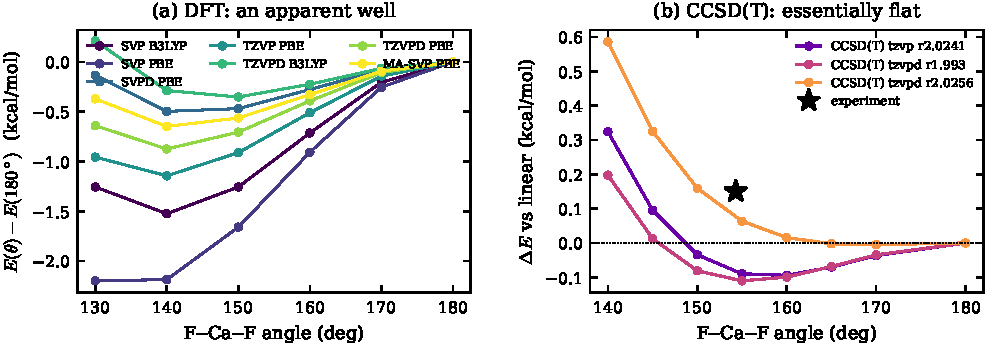
\includegraphics[width=\textwidth]{fig_caf2_bend}
\caption{Bending potential of gas-phase CaF$_2$, both panels relative to the
linear geometry so the two energy scales are comparable. (a) Seven DFT levels,
all producing a well of depth $1.1$ to $2.2$~kcal\,mol$^{-1}$ near
$140^\circ$. (b) CCSD(T) at two basis sets and two Ca--F distances; the well is
$0.05$ to $0.11$~kcal\,mol$^{-1}$ deep and the minimum lies between $155^\circ$
and $170^\circ$, bracketing the experimental $154.3^\circ$. The bending is real;
its depth at DFT is an artefact.}
\label{fig:caf2-bend}
\end{figure}

\begin{figure}[t]
\centering
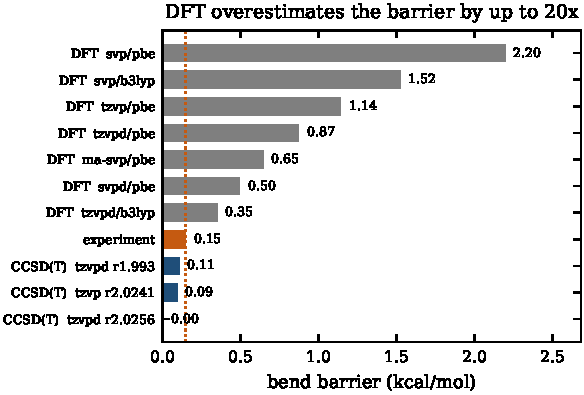
\includegraphics[width=\columnwidth]{fig_barrier_bar}
\caption{Bend barrier for the same molecule at every level computed, against the
experimental $0.15$~kcal\,mol$^{-1}$ (dotted). DFT overestimates by up to a
factor of $20$, improving monotonically with basis size, while the correlated
values sit on or below the experimental bar.}
\label{fig:barrier-bar}
\end{figure}

\begin{figure}[t]
\centering
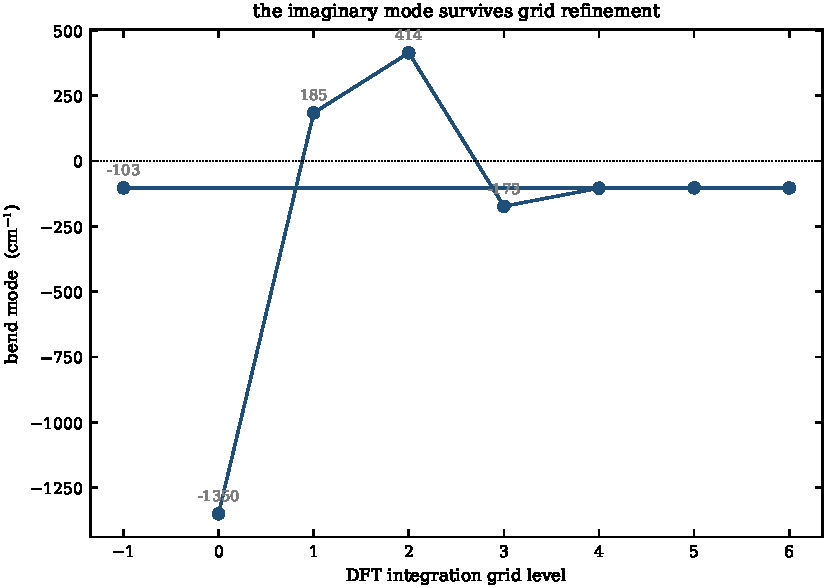
\includegraphics[width=\columnwidth]{fig_grid_convergence}
\caption{The imaginary bend frequency against the DFT integration grid. Levels
one to three disagree in sign, which is what a grid artefact looks like; from
level four onward the value is stable near $-102$~cm$^{-1}$. The mode is
therefore physical for the linear geometry, and the linear geometry is a saddle
at these levels.}
\label{fig:grid-convergence}
\end{figure}

That bound is what the reaction energy needs, because it settles what the
bent-versus-linear column of the table below means. At a correlated level the two
structures differ by at most $0.15$~kcal\,mol$^{-1}$, so the $0.1$ to $2.3$ span that
column shows at DFT levels is method error, not structural uncertainty. We keep both
columns because the calculation was done that way, but the true structural freedom is
ten times smaller than the table suggests.

Two internal checks say the $128.2^\circ$ structure we previously reported should
not be quoted at all. Its gradient norm was $3.0\times10^{-2}$~Ha\,\AA$^{-1}$ ---
not, as we first supposed, a spurious rigid-body force, since switching on the
grid-response term moves the net force from $3.5\times10^{-5}$ to $10^{-14}$ while
leaving the norm unchanged. It was a genuine failure of the optimiser, which was
seeded with $0.3\,I$, roughly $740$ times too stiff along a mode of curvature
$4.1\times10^{-4}$, so no secant pair ever carried bending character. And its
geometry is inconsistent with its own Hessian: a quartic well of that curvature and
$2.06$~kcal\,mol$^{-1}$ depth bottoms at $\approx161^\circ$, while a
$128^\circ$ minimum of that depth would need an imaginary frequency near
$54$~cm$^{-1}$. The angle, the depth and the imaginary frequency cannot all come
from one smooth potential.

The reaction energy is therefore reported twice below, once with $\mathrm{CaF_2}$
at its unconstrained minimum and once constrained to \begin{figure}[t]
\centering
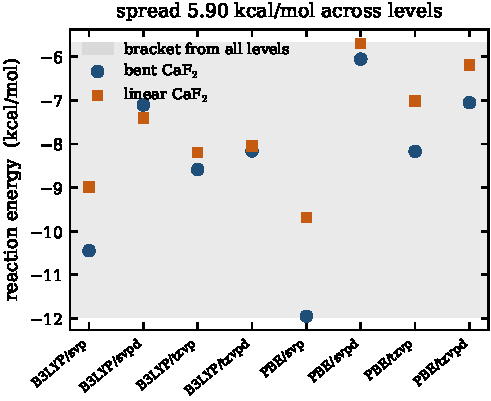
\includegraphics[width=\columnwidth]{fig_reaction_bracket}
\caption{Reaction energy for
$\mathrm{Ca(formamidinate)_2+2HF\to CaF_2+2\,formamidine}$ across eight
functional/basis combinations, with CaF$_2$ either at its unconstrained minimum
or constrained to $D_{\infty h}$. The shaded band is the bracket the paper
reports; the spread across levels, not the value at any one level, is the
honest uncertainty.}
\label{fig:reaction-bracket}
\end{figure}

$D_{\infty h}$, which brackets
the treatment.

\begin{remark}[Why this number must not be quoted as the ALD protonation energy]
Four limitations apply, and none is a technicality.
\begin{enumerate}
\item \emph{Truncated ligand.} Di-\emph{i}-propyl and hydrogen differ by
twenty-four carbon atoms. Substituent effects on a protonation energy of an
amidine are real, and no error bar for the truncation is available here.
\item \emph{Gas phase.} The protonation occurs on a $\mathrm{CaF_2}(111)$ surface
with HF adsorbed at $E_{\mathrm{ads}} \in[-0.62,-0.40]$~eV, not in vacuum. Surface
and co-adsorption effects are absent.
\item \emph{$\Delta E$, not $\Delta G$.} No zero-point, thermal, or entropic
correction is included, so this is not a free energy. An amidine carries two extra
protons on its nitrogen atoms and its desorption entropy is substantial.
\item \emph{No barrier.} A reaction energy says nothing about whether the step
proceeds at $175$--$250$~$^\circ$C. Section~\ref{sec:worked} proved that a barrier
cannot be bounded above by configuration sampling at all, so this number cannot be
converted into a rate.
\end{enumerate}
What the calculation does establish is narrower and still useful: the
ligand-protonation stoichiometry is thermodynamically downhill for the amidinate
core, by of order ten kcal\,mol$^{-1}$, with a method spread small compared to the
effect. That is consistent with the protonation mechanism inferred from the
fluoride ALD literature and inconsistent with an endothermic step.
\end{remark}

\subsection{What remains open for this system}

\begin{enumerate}
\item The elementary-step mechanism and any activation energy for
HF reacting with an adsorbed calcium amidinate on $\mathrm{CaF_2}(111)$. No
value is available in the sources consulted, and Theorem~\ref{thm:nosampling}
shows that a barrier can be certified from below only.
\item The ligand footprint $A_0$ of di-\emph{i}-propylformamidinate, which
Theorem~\ref{thm:footprint} needs in order to become a quantitative cap.
\item Whether the observed $9.51$--$12.68\%$ coverage reflects steric
self-limitation or kinetics. Distinguishing them requires a coverage-dependent
measurement, not a bound.
\item The substrate relationship, which is deliberately absent here. If growth
continues on existing $\mathrm{CaF_2}$ the relevant surface is $\mathrm{CaF_2}$;
the role of an underlying Si(100) is epitaxial orientation, not surface
chemistry. The orientation question is not vacuous: the epitaxial literature
reports $\mathrm{CaF_2}$ growth overwhelmingly on Si(111), where the lattice
mismatch is only $0.6\%$ at room temperature and $1.6\%$ at $600$~$^\circ$C
\citep{Pilvi2007}, and reports $\mathrm{CaF_2}$-(110) rather than (100) on
Si(001); epitaxial overgrowth restricted to (111) orientations is likewise
documented on the fluoride side \citep{Chan2010}. A Si(100) substrate therefore
does not inherit the (111) orientation
result, and we do not assume it does.
\item The quantitative bending potential of gas-phase $\mathrm{CaF_2}$. That the
linear geometry is a saddle is settled: it is quasilinear, and the CCSD(T) barrier
is $0.15$~kcal\,mol$^{-1}$ \citep{Koput2004}. What is not settled is how much of
our computed $2.19$ (PBE/def2-svp) is basis error. Diffuse and higher-$d$ bases
bring it to $0.29$--$0.87$ depending on functional and level, still above the
reference, and a CCSD(T) focal-point optimisation of the three-atom molecule is the
one calculation that would close it. That is affordable and not done here.
\end{enumerate}

The honest summary of this section is therefore narrow and two-part. On the process
side, two published numbers plus a lattice constant fix the fractional coverage of
a cycle and show that site availability is not the limiter; a kernel-checked
inequality turns that into a ligand-design cap, and a kernel-checked counterexample
shows that the barrier for the same system cannot be bounded above by any amount of
configuration sampling. No barrier value for this system is claimed.

On the electronic side, one result now exists: the model protonation reaction is
exothermic by $5.7$--$12.0$~kcal\,mol$^{-1}$ across eight levels and two
$\mathrm{CaF_2}$ treatments, narrowing to $-6$ to $-8$ at the four levels we
consider adequate. It is a bracket, not a number, and the remark above lists four
reasons it is not the ALD protonation energy. What it does establish is that the
arithmetic of the certificate chain can be carried through a real integral set at
verified minima, and what it exposes is which input is missing next.
